\section{Classification \& Bio-geophysical Parameter Retrieval}

\subsection{Can we predict where there is chlorophyll through classification?}

We will use \textit{K-Means clustering} to classify the data. K-means clustering is a 
unsupervised learning algorithm that can be used to classify and cluster data into $k$ 
different clusters. The data points are adjusted iteratively until all points are 
associated with the nearest cluster. We want to cluster each observation (pixels, with $n$ spectral channels) into a specific 
cluster (environment class, ie. deep water, shallow water, vegetation). 


\begin{figure}
    \centering
    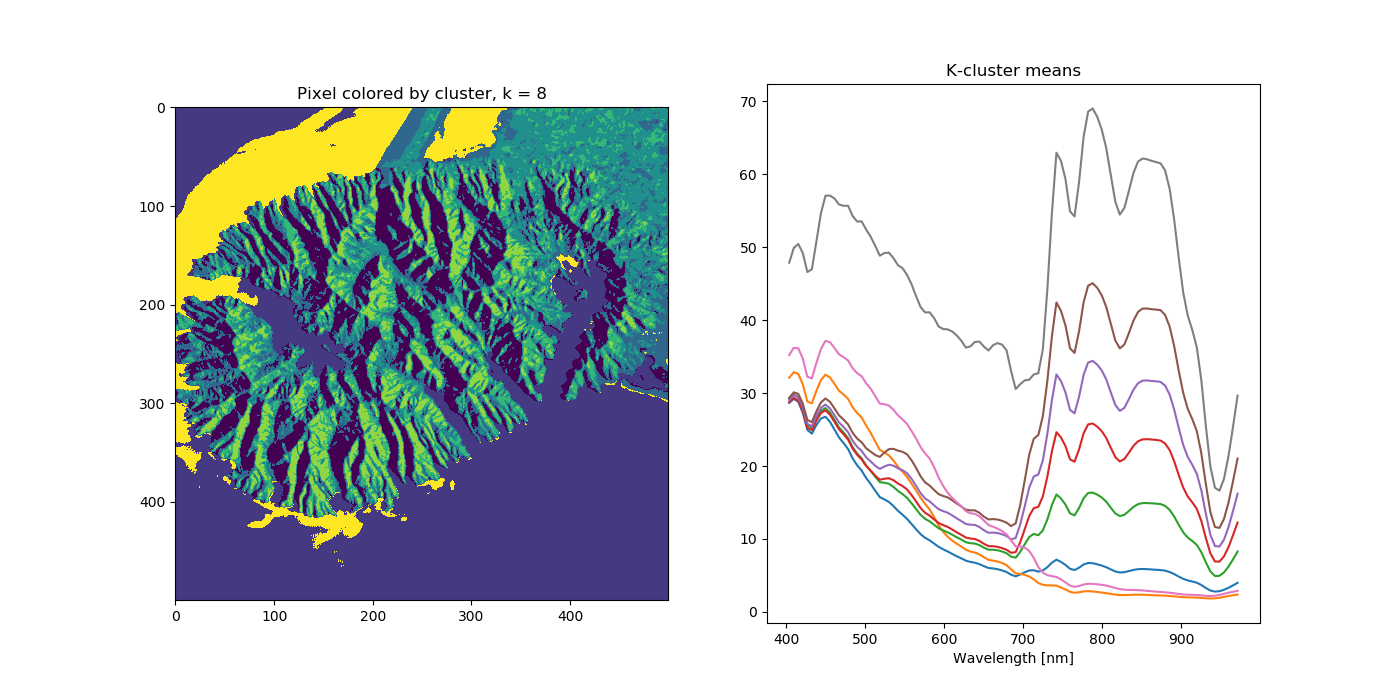
\includegraphics[width=\textwidth]{../fig/kmean/kmean_8.png}
    \caption{K-mean clusters of the image}
    \label{fig:kmean}
\end{figure}

As we can see from \cref{fig:point_spectra}, we know that those three different points 
have distinctly different spectra, thus it should be possible to classify them accordingly. 
The results of a K-mean clustering, run with Spectral Python's \textit{kmeans} function \cite{website:spectral}, 
can be seen in \cref{fig:kmean}. We clearly see different classes for water, land, and vegetation, the latter 
containing lots of chlorophyll. We also see a very distinct class along the coast on the upper part 
of the image. This may very well be a collection of chlorophyll, but it might also just be shallow water, or 
more likely a combination of both. 

\subsection{How well can we directly estimate the chlorophyll content?}

We use the NASA OBPG algorithm, defined in equation 4 in the assignment 
\cite{assignment}, as well as the parameters given there, to try to 
visualize the chlorophyll contents. Using the closest available wavelengths 
in the dataset, $\lambda_{green} = 553$ (i = 26) and $\lambda_{blue} = [444, 490, 507]$ 
(i = [7, 15, 18]). The results can be seen in \cref{fig:obpg}. We can clearly 
see high concentrations on the north west coast, same place as in \cref{fig:kmean}, 
but now we also see quite a bit on the southern coast as well. Thus it seems that this 
algorithm performs better than the k-means clustering. 

\begin{figure}
    \centering
    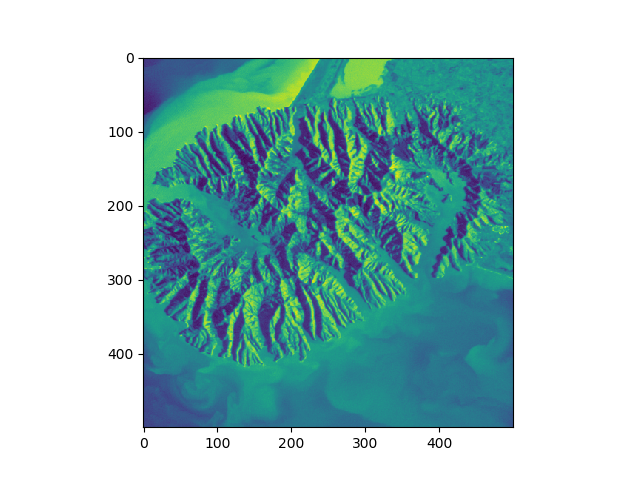
\includegraphics[width=\textwidth]{../fig/2b_nasa.png}
    \caption{Results from the NASA OBPG algorithm, showing chlorophyll concentrations}
    \label{fig:obpg}
\end{figure}

\subsection{How can we estimate the reflectance from the surface of the ocean?}

\subsection{Compute chlorophyll concentration using atmosphere-corrected data}

\subsection{Classify land versus water}

\subsection{Other bio-geophysical parameters}

\subsection{Alternative atmospheric correction methods}